\documentclass{article}
\usepackage[utf8]{inputenc}
\usepackage{amsmath}
\usepackage{amsfonts}
\usepackage{tabularx}
\usepackage{layout}
\usepackage{geometry}
\usepackage{siunitx}
\usepackage{calc}
\usepackage{siunitx}
\usepackage{graphicx}
\usepackage{listings}
\usepackage{xcolor}
\usepackage{longtable}
\usepackage{soul}
\usepackage{float}
\usepackage{calligra}
\usepackage{mathtools}
\usepackage{physics}

\setlength{\hoffset}{0in}
\setlength{\voffset}{0in}
\setlength{\oddsidemargin}{0px}
\setlength{\headheight}{0em}
\setlength{\headsep}{0em}
\setlength{\marginparwidth}{0em}
\setlength{\marginparsep}{0em}
\setlength{\textheight}{\paperheight - 2in}
\setlength{\textwidth}{\paperwidth - 2in}
\setlength{\parskip}{1.5em}

\setlength{\parindent}{0px}
\setlength{\parskip}{2em}
\setlength{\tabcolsep}{0.2em}

\newcolumntype{C}{>{\centering\arraybackslash}X}

\newcommand{\expart}[1]
{
    \textbf{\underline{#1:}} \par 
}

% Unités
\newcommand{\un}[1]{
    \,\text{#1}
}

\newcommand{\question}[2]
{
    \begin{tabularx}{\linewidth}{lX}
        \textbf{#1)} & {#2}
    \end{tabularx} 
}

\begin{document}

Chollet Arthur

\begin{center}
  \Huge
  \normalfont\calligra Compte-rendu de capacité numérique
\end{center}

\expart{6.1 Vérification de la deuxième loi de Kepler}

\question{1}{
  En identifiant les coordonnées sphériques avec: $\boldsymbol{r}$: l'altitude + $R_T$, $\boldsymbol{\theta}$: la longitude et $\boldsymbol{\varphi}$: la latitude. On obtient que:
  $$
  \boxed{\begin{cases}
    x=r\sin\theta\cos\varphi\\
    y=r\sin\theta\sin\varphi\\
    z=r\cos\theta\\
  \end{cases}}
  $$
}

\question{2}{
  La méthode de dérivation utilisée est:
  \begin{itemize}
    \item pour le 1er élément:
    $$
      v=\frac{OM_1-OM_0}{t_{1}-t_{0}}
    $$
    \item pour les éléments centraux (meilleure approximation):
    $$
      v=\frac{OM_{i+1}-OM_{i-1}}{t_{i+1}-t_{i-1}}
    $$
    \item pour le dernier élément:
    $$
      v=\frac{OM_{i}-OM_{i-1}}{t_{i}-t_{i-1}}
    $$
\end{itemize}
}

\question{3}{
\begin{figure}[H]
  \centering
  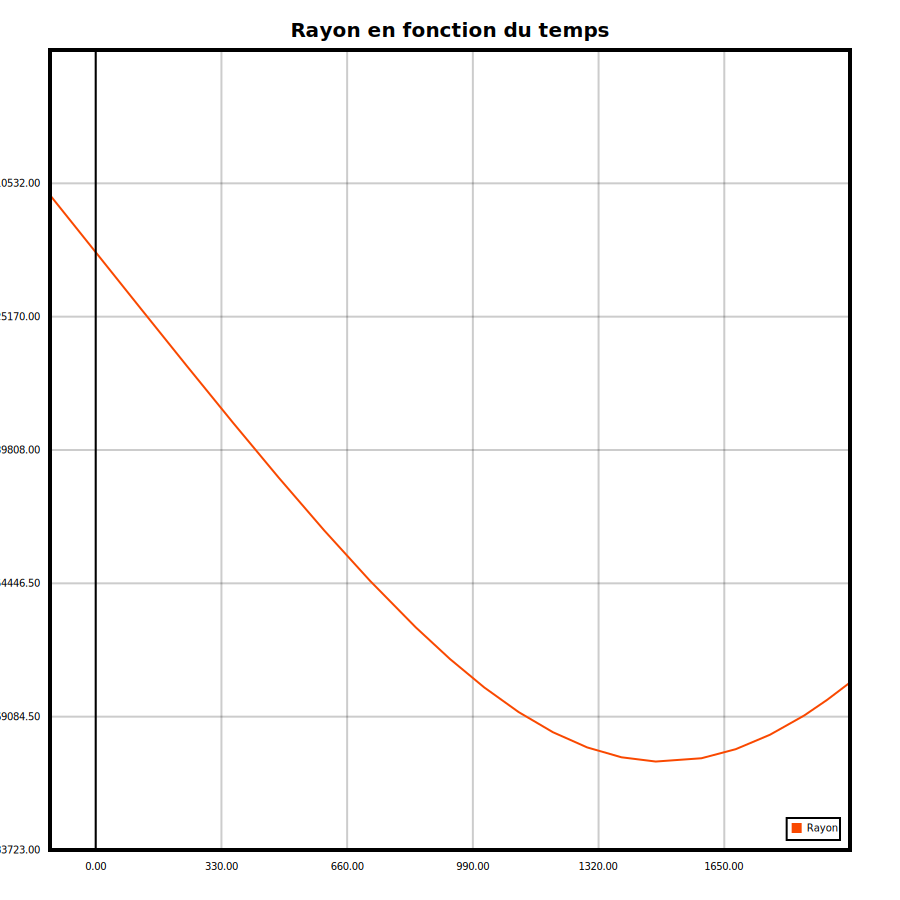
\includegraphics[width=50mm]{img/radius.png}
  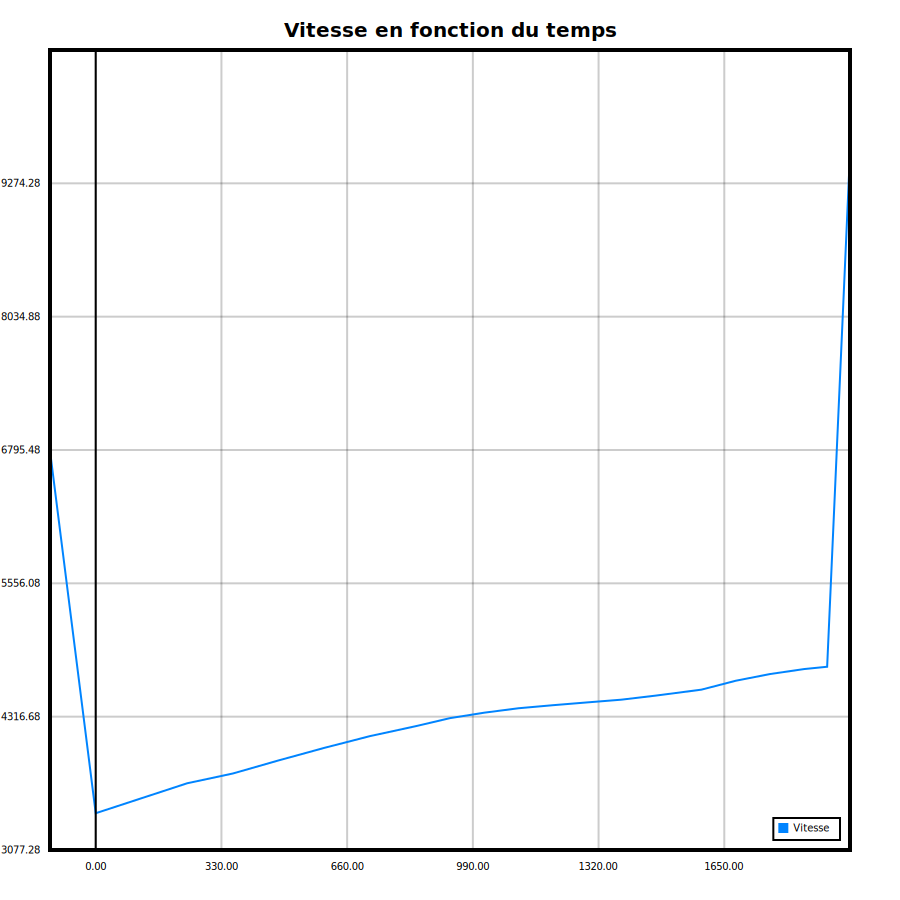
\includegraphics[width=50mm]{img/velocity.png}
  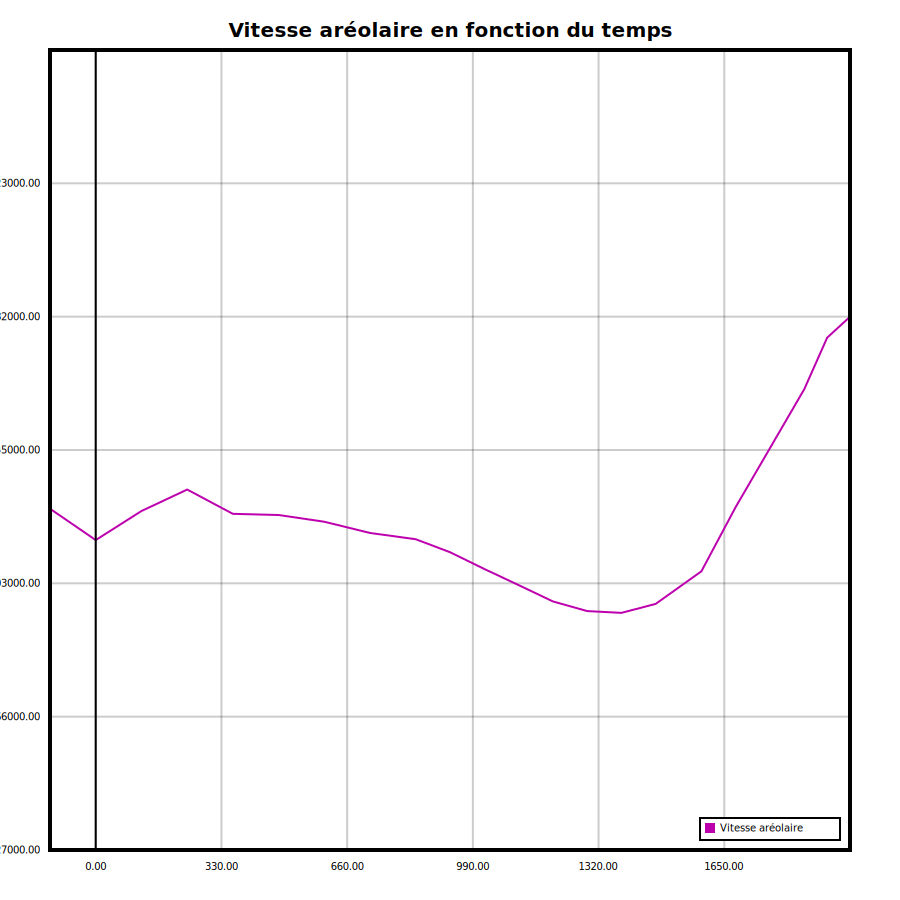
\includegraphics[width=50mm]{img/areal_velocity.png}
  \caption{Tracé du rayon (orange), de la vitesse (bleu) et de la vitesse aréolaire (violet) en fonction du temps}
\end{figure}
À noter que pour la vitesse, le premier et le dernier point ne sont pas cohérents au vu de la méthode de dérivation spéciale utilisée.
}

\question{4}{
  La deuxième loi de Kepler nous dit que pour un intervalle de temps égal, l'aire parcourue par le satellite est constante. Dans nos données, nous avions trois régimes d'intervalles de temps différents : de -2 min à 14 min avec un intervalle de 2 min, de 14 min à 31 min avec un intervalle de 1,5 min, puis de 31 min à 33 min avec un intervalle de 1 min. On identifie sur la courbe de la question 3 des courbes constantes (au vu de l'ordre de grandeurs et de l'échelle) pour chacun de ces intervalles (les variations étant dues aux transitions d'intervalles). On conclut ainsi que \underline{la deuxième loi de Kepler est vérifiée}.
}

\expart{6.2 Vérification de la troisième loi de Kepler}

\underline{Système}: Étoiles orbitant autour de Sagittarius $A^*$

\underline{Référentielle}: centré sur Sagittarius $A^*$

\question{1}{
  Nous traçons à partir des valeurs de $\boldsymbol{a}$ et $\boldsymbol{T}$ la courbe $a^3=f(T^2)$ et cherchons à identifier la nature de $\boldsymbol{f}$
  \begin{figure}[H]
    \centering
    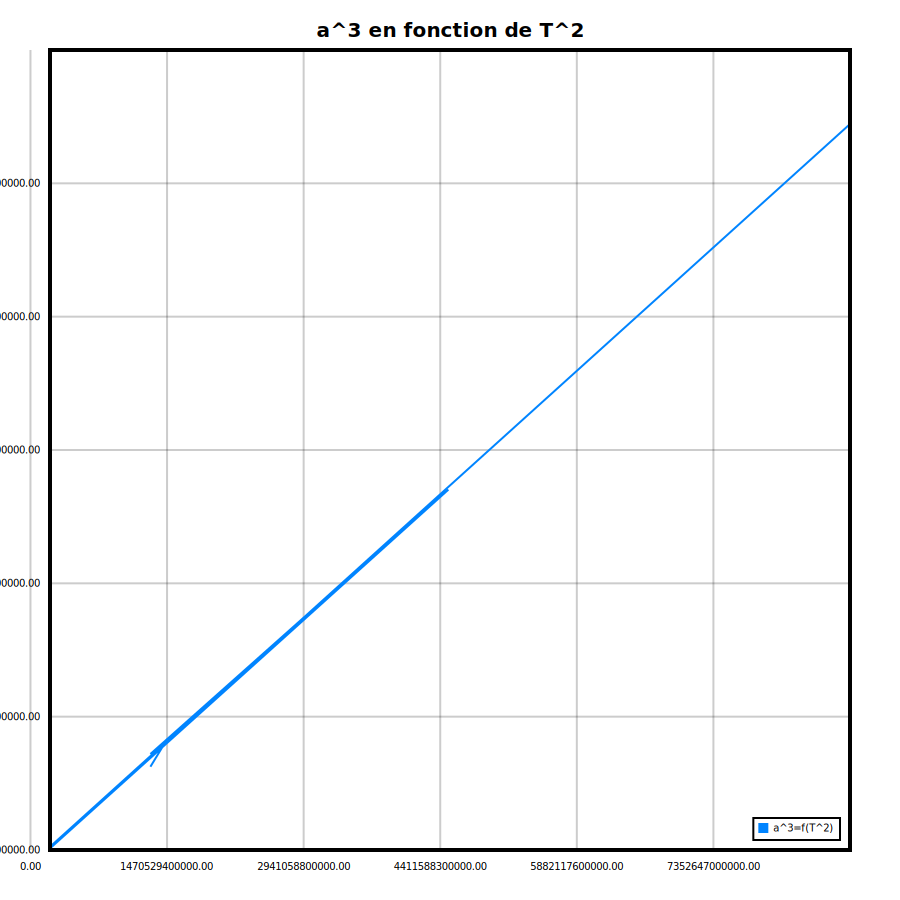
\includegraphics[width=50mm]{img/third_law.png}
    \caption{Tracé de $a^3$ en fonction de $T^2$}
  \end{figure}
  On identifie ainsi une fonction affine, et par régression linéaire sur les données obtenues : $a^3=1,366.10^{25}\times T^2+b$ (avec $b\ll10^{25}$).

  On conclut ainsi que 
  $$\boxed{\frac{a^3}{T^2}=(1.366\pm0.058).10^{25} m^3s^{-2}=\text{constante}}$$  ce qui valide la troisième loi de Kepler pour Sagittarius $A^*$
}

\question{2}{
  Or on sait que:
  $$
  \frac{a^3}{T^2}=\frac{GM_{TN}}{4\pi^2}
  $$
  donc
  $$
  \boxed{M_{TN}=\frac{4\pi^2a^3}{GT^2}}
  $$
  Soit en application numérique: $\boxed{M_{TN}=(8.08\pm0.37).10^{36} \un{kg}}$
}

\question{3}{
  On applique la formule:
  $$
    z=\frac{\abs*{M_{TN}-M_{TN,tab}}}{\sigma}=\frac{8.2541-8.08}{0.37}=0.47 < 2
  $$

  Le \underline{z-score est inférieur à 2}, on conclut donc que nos mesures sont cohérentes.
}

\end{document}
